\chapter{Umsetzung} %Beide

\section{Umsetzung der Anwendung} %Benedikt

\section{Umsetzung des künstlichen neuronalen Netzes mit Neurophstudio} %Sebastian
\label{section:Umsetzung des künstlichen neuronalen Netzes mit Neurophstudio} %Sebastian

In diesem Abschnitt wird beschrieben, wie das \acs{knn} aus der Konzeptionsphase umgesetzt wurde. Zum Umsetzung wurde Neurophstudio verwendet. Neurophstudio ist ein Teil von Neuroph und erlaubt das Erstellen, Trainieren sowie Testen von \acs{knn}.
Nachdem das \acs{knn} angelegt wurde, musste es noch trainiert und anschließend getestet werden. Für diesen Vorgang sind Trainings- sowie Testdaten zur nötig. Die benötigten Daten konnten als Excel-Datei von der nachfolgenden Webseite bezogen werden: 
\textit{http://www.quandl.com/}. Es wurden die letzten 600 Datensätze extrahiert und dann in 2 Datensätze aufgeteilt: Einen Datensatz bestehend aus 450 Trainingsdaten sowie einen Datensatz bestehend aus 150 Testdaten.Da diese Datensätze noch nicht normalisiert waren, die Daten jeodch in normalisierter Form für das \acs{knn} zur Verfügung stehen müssen, wurden diese mit folgender Formel normalisiert:

\begin{equation}\formelentry{Normalisierungsformel}
  N_h = \frac{A-min(A}{max(A)-min(A)}\cdot0,8+01
\end{equation}

Mit Hilfer dieser Normalisierungsformle ist sichergestellt, dass sich alle WErte der Datensätze im Intervall $[0,1]$ befinden,wobei die Multiplikation mit $0,8$ sowie die Addition mit $0,1$ Extremwerte abmildern soll.

Nachdem alle Komponenten für die Erstellung eines fertigen \acs{knn} vorhanden waren, konnte mit dem Training begonnen werden. Dafür wurden $200.000$ Trainingszyklen gestartet und mit einer Lernrate von $0,7$ verwendet. Dieser Wert hat sich als ein guter Startwert herausgestellt.


\section{Optimierung des künstlichen neuronalen Netzes}

Nachdem das Grundmodell des \acs{knn} Funktionsfähig war, wurde dieses noch weiter optimiert, darauf wird nun in den folgenden Unterabschnitten genauer eingegangen. 

\label{section:Optimierung des künstlischen neuronalen Netzes}
\subsection{Optimierung der Topologie}
Das im Abschnitt \ref{section:Umsetzung des künstlichen neuronalen Netzes mit Neuroph} wird in diesem Abschnitt hinsichtliche der verwendeten Topolgie optimiert. Dabei wurden mit der Topologie begonnen und sukzessive Neuronen in der Zwischenschicht hinzugefügt bzw. weggenommen und für jeden Trainings- und Testverlauf der MSE notiert. die Topologie mit den geringsten MSE im Testverlauf wurde dann übernommen. DIe ERgebniss können aus der folgenden Tabelle ebtnommen werden:


\begin{table}[H]
  \centering
  \begin{tabular}{|c|c|c|}
  \hline 
  \rule[0ex]{0pt}{2.5ex} Topologie & Training-MSE & Test-MSE \\ 
  \hline 
  \rule[0ex]{0pt}{2.5ex} 4-05-1 & 0.000 & 0.000 \\ 
  \hline 
  \rule[0ex]{0pt}{2.5ex} 4-07-1 & 0.000 & 0.000 \\ 
  \hline 
  \rule[0ex]{0pt}{2.5ex} 4-11-1 & 0.000 & 0.000 \\ 
  \hline 
   \rule[0ex]{0pt}{2.5ex} 4-01-1 & 0.000 & 0.000 \\ 
  \hline 
  \rule[0ex]{0pt}{2.5ex} 4-14-1 & 0.000 & 0.000 \\ 
  \hline 
  \rule[0ex]{0pt}{2.5ex} 4-17-1 & 0.000 & 0.000 \\ 
  \hline 
  \end{tabular} 
  \caption{Jeweilige Topologien \& korrespondierende MSE}
  \label{tab:TOPMSE}
\end{table}


Demnach wird die neue Topologie des \acs{knn} mit sieben Neuuronen in der versteckten Schicht arbeiten.



\subsection{Wahl der optimalen Transferfunktion} 
\label{subsection:Wahl der optimalen Transferfunktion} 


\begin{figure}[H]
\hfill
\subfigure[Sigmoid]{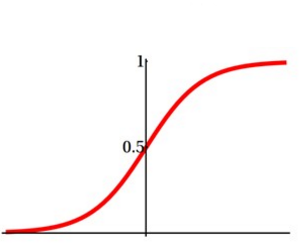
\includegraphics[width=5cm]{Sigmoid.PNG}}
\hfill
\subfigure[Tanh]{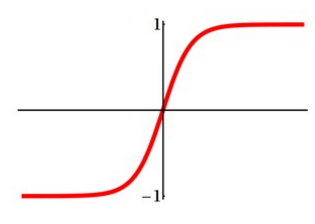
\includegraphics[width=5cm]{tanh.PNG}}
\hfill
\caption{Die Sigmoide Funktion und die Tanh Funktion im Vergleich}
\end{figure}


\begin{equation}\formelentry{Sigmoide Funktion sowie Tanh Funktion}
(a)\ f(x)= \frac{1}{1+e^{-cx}}\ \ \ \ \ \ \ \ \ \ \ (b)\ f(x)= tanh(x)
\end{equation}

Das \acs{knn} wurde einmal mit einer Sigmoiden Funkiton trainiert und getesten und anschließend nochmas mit einer Tanh Funktion trainiert und geteste. Die Ergebnisse können aus der untenstehnen Tabelle entnommen werden:

\begin{table}[H]
  \centering
  \begin{tabular}{|c|c|}
  \hline 
  \rule[0ex]{0pt}{2.5ex} Transferfunktion & Mean Squared Error \\ 
  \hline 
  \rule[0ex]{0pt}{2.5ex} Sigmoid & 0.000 \\ 
  \hline 
  \rule[0ex]{0pt}{2.5ex} Tanh & 0.000 \\ 
  \hline 
  \end{tabular} 
  \caption{Jeweilige Transferfunktionen \& korrespondierende MSE}
  \label{tab:TRANSMSE}
\end{table}

\subsection{Wahl der optimalen Lernregel} %Sebastian

Innerhalb des Verfahrens der überwachten Lernens existieren mehrere Lernregeln, um das Netz zu trainieren. Die bekannteste Lernregel dürfte hier das Backpropagation sein. Diese Regel gibt es ebenfalls in mehreren Variationen wie das momentum Backpropagation sowie das Resilient Backpropagation. Diese Fehlerrückführungsverfahren werden nun jeweils einzeln beschrieben und anschlißedend genauer analysiert und das für die Anweungs am besten geeignstete Verfahren ausgewählt.

\begin{itemize}
\item Backpropagation: Dies ist das klassische Fehlerrükcführungsverfahren zum Anpassen der Verbindungsgewichte. Die Gewichtsveränderung erfolgt durch einen Fehlersignal, dass aus der Abweichung von tatsächlicher und prognostizierter Ausgabe berechnet wird. Die Gewichtsveränderung erfolgt hierbei schichtweise von den Ausgangsneuronen bis zu den Eingangneuronen.

\item Momentum Backpropagation: Dieses Backpropagationverfahren fügt dem klassichen Verfahren einen Trägheitsterm hinzu, indem die Gewichtsveränderung zum Zeitpunkt $t-1$ berücksichtigt wird. Der Momentumwert gibt dabei die Sträkre an, wie startk dieser Wert berücksichtigt wird (zwischen 0 und 1).Durch diesen Trägheitsterm wird die Wahrscheinlichkeit, dass das \acs{knn} beim Training in ein lokales Minimum oszilliert und sich somit nicht weiter den Idealwert approximieren kann. Auch die Wahl der Lernrate gestaltet sich hier weniger kritisch. 

\item  




Zur Bestimmung des Fehlers zwischen der prognostizierten and tatsächlichen Ausgabe kann der MSE benutzt werden. Die MSE-Formel würde in den konkreten Fall der Anwendung wie folgt lauten:

\begin{equation}\formelentry{MSE zur Berechnung der Abweichung}
   \frac{1}{2}\sum^{n}_{i=1} (KT_{i} - KV_{i})^2
\end{equation}

Wobei $n$ für die Anzahl der Datensätze steht, $KT_i$ für den tatsächlichen Ausgabewert für den Datensatz $i$ steht und $KV_i$ für den prognostizierten Datensatz $i$ steht.

\end{itemize}



\begin{table}[H]
  \centering
  \begin{tabular}{|c|c|c|}
  \hline 
  \rule[0ex]{0pt}{2.5ex} Lernregel & Mean Squared Error \\ 
  \hline 
  \rule[0ex]{0pt}{2.5ex} Backpropagation & 0.000 \\ 
  \hline 
  \rule[0ex]{0pt}{2.5ex} Momentum Backpropagation & 0.000\\ 
  \hline 
  \rule[0ex]{0pt}{2.5ex} Resilient Propagation & 0.000 \\ 
  \hline 
  \end{tabular} 
  \caption{Jeweilige Lernregeln \& korrespondierende MSE}
  \label{tab:tab3}
\end{table}



\section{Die endgültigen künstlichen neuronalen Netze}
<<Sebastian>> \Blindtext
\section{Zusammenführung der Komponenten}
<<benedikt>> \Blindtext
